\documentclass[10pt]{beamer}

% Konfiguracja języka i fontów
\usepackage[T1]{fontenc}
\usepackage[utf8]{inputenc}
\usepackage[polish]{babel}
\usepackage{lmodern}
\usepackage{booktabs}
\usepackage{graphicx}
\usepackage{amsmath}
\usepackage{amsfonts}

% motyw
\usetheme{Madrid}
\setbeamertemplate{frame numbering}[fraction]
\usecolortheme{crane}

\title{Analiza stabilności numerycznej algorytmów na przykładzie obliczania wartości funkcji pierwiastkowych}
\subtitle{Metody Obliczeniowe w Nauce i Technice}
\author{Piotr Sączawa}
\date{\today}

\begin{document}

% Slajd 1: Tytułowy
\begin{frame}
    \titlepage
\end{frame}

% Slajd 2: Cel doświadczenia
\begin{frame}{Cel doświadczenia}
    \begin{itemize}
        \item Analiza porównawcza dwóch matematycznie tożsamych sformułowań funkcji:
        \begin{equation*}
            f(x) = \sqrt{x^2 + 1} - 1, \quad g(x) = \frac{x^2}{\sqrt{x^2 + 1} + 1}
        \end{equation*}
        \item Wyznaczenie wpływu skończonej precyzji arytmetyki zmiennoprzecinkowej (IEEE 754) na wynik obliczeń.
        \item Porównanie zachowania typów \texttt{float}, \texttt{double} oraz \texttt{long double}.
        \item Badanie stabilności dla argumentów skrajnych ($x \to 0$ oraz $x \to \infty$).
    \end{itemize}
\end{frame}

% Slajd: Architektura i środowisko eksperymentalne
\begin{frame}{Środowisko eksperymentalne i architektura}
    \begin{block}{Specyfikacja techniczna}
        \begin{itemize}
            \item \textbf{System operacyjny:} Windows 11.
            \item \textbf{Procesor:} Architektura x86\_64 (obsługa jednostek FPU i instrukcji SSE/AVX).
            \item \textbf{Kompilator C++:} GCC (MinGW-w64) -- standard C++17.
            \item \textbf{Środowisko obliczeniowe Python:} Python 3.15 (biblioteki: \texttt{pandas}, \texttt{matplotlib}, \texttt{numpy}).
            \item \textbf{Referencja wysokiej precyzji:} Biblioteka \texttt{decimal} (ustawiona precyzja: 100 cyfr znaczących).
        \end{itemize}
    \end{block}
    
    \begin{alertblock}{Uwaga dot. typu \texttt{long double}}
        W użytej architekturze (x86\_64) i kompilatorze GCC, typ \texttt{long double} zajmuje zazwyczaj 12 lub 16 bajtów w pamięci, oferując 80-bitową precyzję (rozszerzony format x87), co pozwala na dokładniejszą analizę błędów typu \texttt{double}.
    \end{alertblock}
\end{frame}

% Slajd 3: Teoria - Katastrofalne obcięcie (Loss of Significance)
\begin{frame}{Problem I: Katastrofalne obcięcie (x $\to$ 0)}
    Dla bardzo małych wartości $x$, wyrażenie $\sqrt{x^2+1}$ dąży do $1$.
    \begin{block}{Mechanizm błędu w f(x)}
        Gdy $x^2 < \epsilon_{machine}$, wartość pod pierwiastkiem jest reprezentowana jako dokładnie $1.0$ ze względu na ograniczoną liczbę bitów mantysy.
        \begin{itemize}
            \item Następuje odejmowanie dwóch bliskich sobie liczb ($1.0 - 1.0$).
            \item Najbardziej znaczące bity wyniku zostają wyzerowane.
            \item Wynik traci wszystkie cyfry znaczące (wynik 0 dla $x \neq 0$).
        \end{itemize}
    \end{block}
    \textbf{Rozwiązanie:} Przekształcenie do postaci $g(x)$ eliminuje odejmowanie w liczniku na rzecz dodawania w mianowniku, co jest operacją stabilną numerycznie.
\end{frame}

% Slajd 4: Teoria - Przepełnienie (Overflow)
\begin{frame}{Problem II: Przepełnienie zakresu (x $\to \infty$)}
    Typy danych IEEE 754 mają ściśle określony zakres wykładnika (cechy).
    \begin{table}[]
        \centering
        \begin{tabular}{@{}lll@{}}
            \toprule
            Typ & Max wykładnik & Max wartość ($x^2$) \\ \midrule
            \texttt{float} (32-bit) & $2^{127}$ & $\approx 3.4 \cdot 10^{38}$ \\
            \texttt{double} (64-bit) & $2^{1023}$ & $\approx 1.8 \cdot 10^{308}$ \\ \bottomrule
        \end{tabular}
    \end{table}
    \begin{itemize}
        \item Dla dużych $x$, operacja $x^2$ może spowodować \textbf{Overflow} ($+\infty$).
        \item W funkcji $g(x)$ prowadzi to do symbolu nieoznaczonego $\frac{\infty}{\infty}$, interpretowanego jako \texttt{NaN}.
        \item \textbf{Optymalizacja:} Dla ekstremalnie dużych $x$ należy stosować przybliżenie asymptotyczne $f(x) \approx x - 1$.
    \end{itemize}
\end{frame}

% Slajd 5: Wyniki - Małe argumenty (Zanik wartości)
\begin{frame}{Wyniki: Zanik wartości funkcji f(x)}
    \begin{figure}
        \centering
        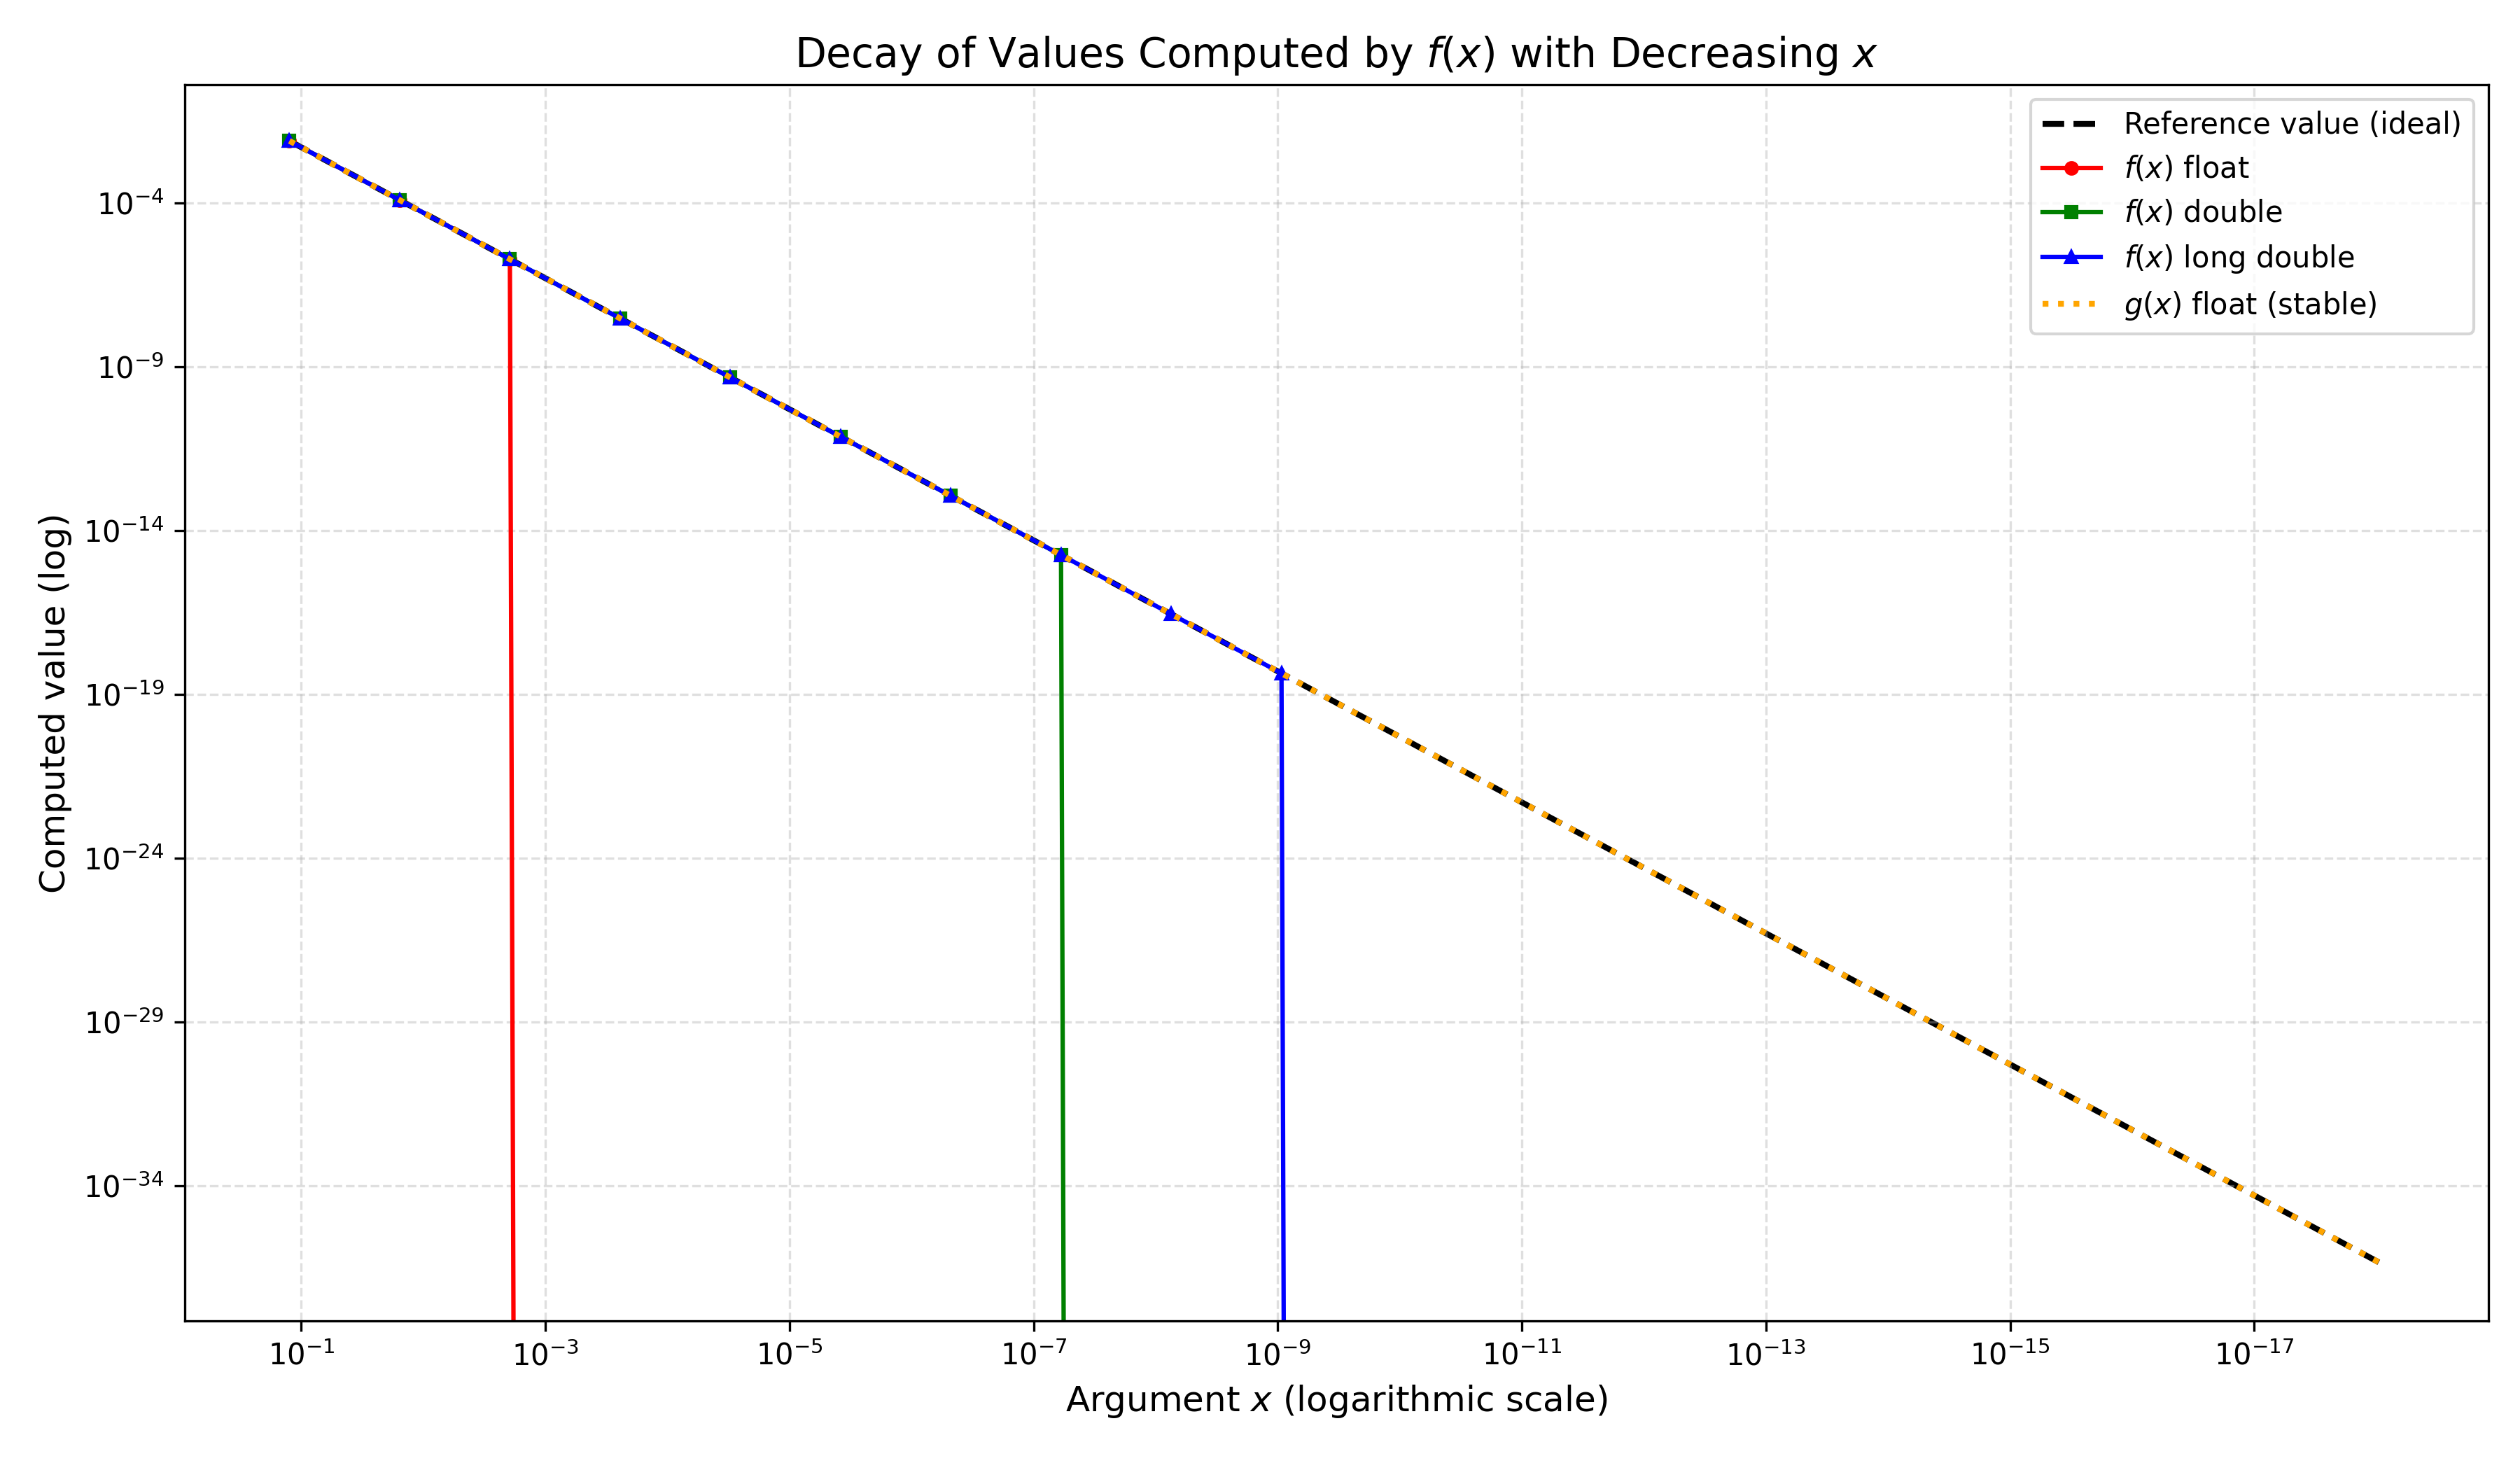
\includegraphics[width=0.85\textwidth]{wykres_zaniku_wartosci.png}
        \caption{Porównanie wartości obliczonych: f(x) vs g(x). Widoczny nagły spadek f(x) do zera.}
    \end{figure}
\end{frame}

% Slajd 6: Wyniki - Analiza błędu względnego
\begin{frame}{Wyniki: Błąd względny}
    \begin{figure}
        \centering
        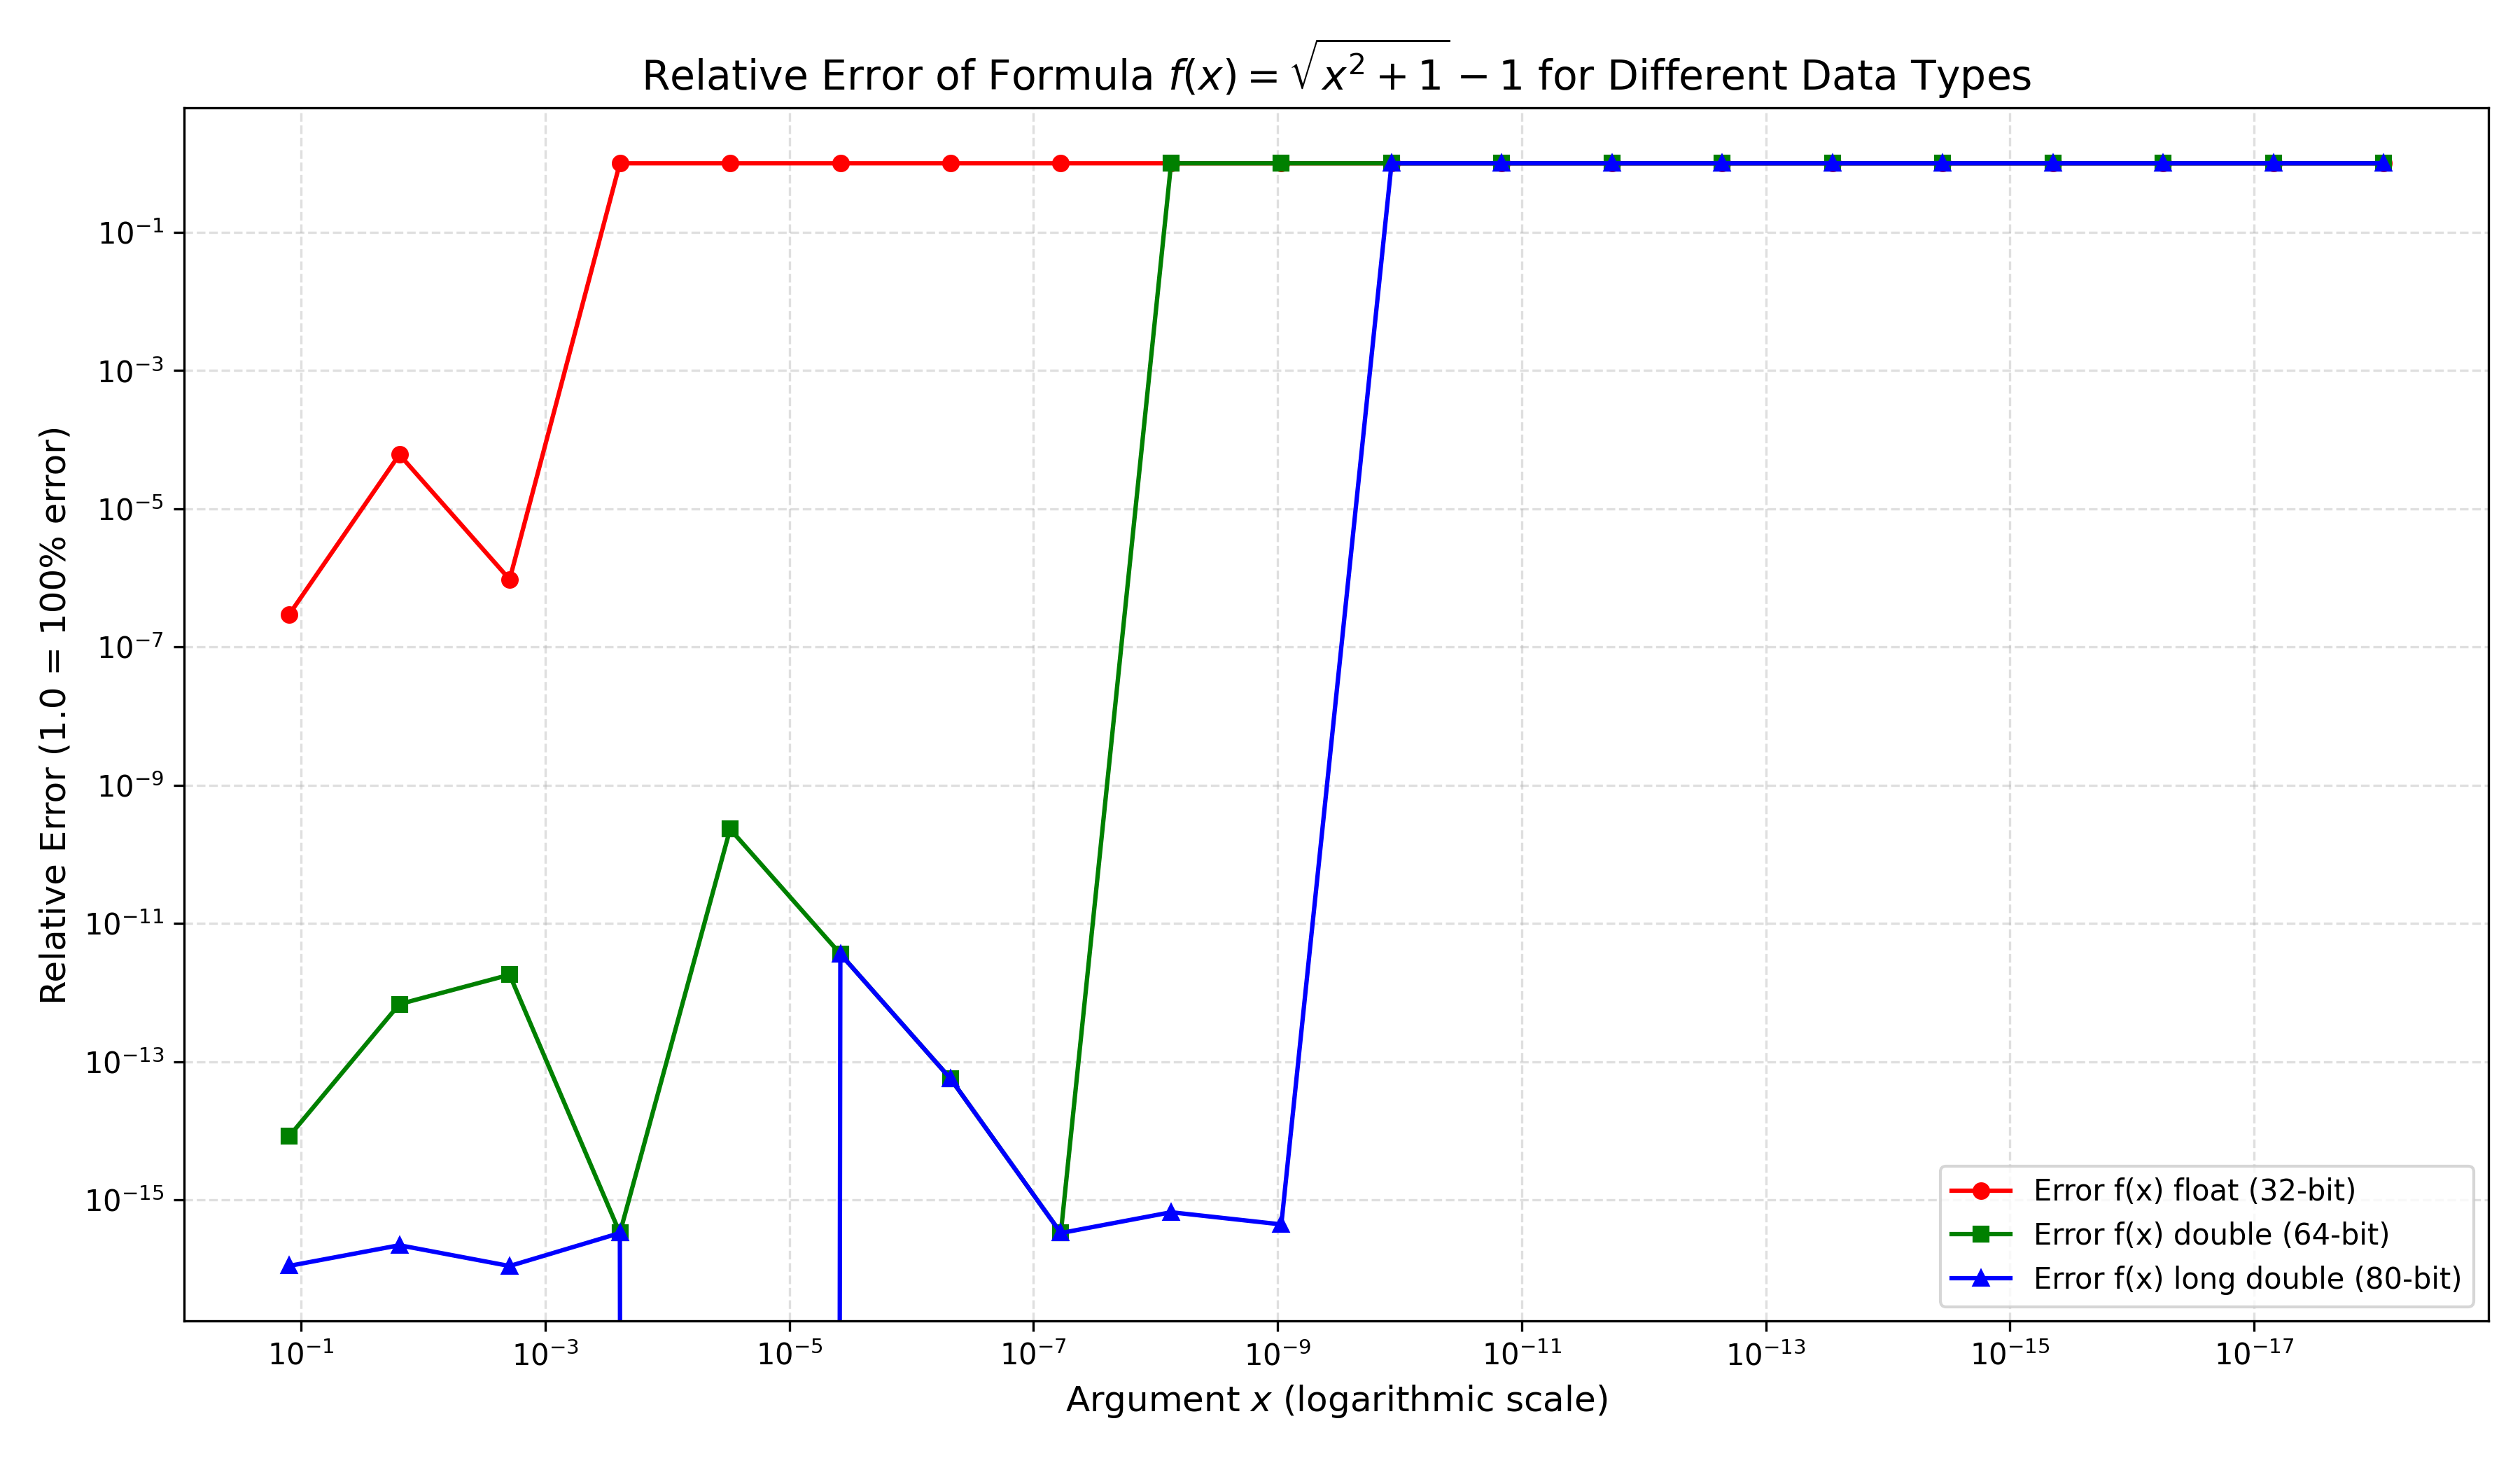
\includegraphics[width=0.85\textwidth]{wykres_bledow_3typy.png}
        \caption{Błąd względny funkcji f(x) narastający wraz ze spadkiem wartości argumentu.}
    \end{figure}
\end{frame}

% Slajd 7: Wpływ precyzji (float vs double)
\begin{frame}{Analiza wpływu precyzji na stabilność}
    Z wykresów wynika wyraźna korelacja między długością mantysy a momentem wystąpienia błędu:
    \begin{itemize}
        \item \textbf{float (23 bity mantysy):} Całkowita utrata precyzji dla $x \approx 10^{-4}$.
        \item \textbf{double (52 bity mantysy):} Stabilność zachowana do $x \approx 10^{-8}$.
        \item \textbf{long double (64/80 bitów):} Najwyższa odporność na błędy zaokrągleń.
    \end{itemize}
    \textit{Wniosek:} Zmiana typu na wyższy jedynie odsuwa problem w czasie, nie rozwiązując niestabilności samego algorytmu.
\end{frame}

% Slajd 8: Duże argumenty - Tabela wyników
\begin{frame}{Zachowanie dla dużych argumentów (Overflow)}
    Wyniki eksperymentalne potwierdzają granice typów:
    \begin{table}[]
        \small
        \centering
        \begin{tabular}{@{}lcccc@{}}
            \toprule
            $x$ & $f\_float$ & $g\_float$ & $f\_double$ & $g\_double$ \\ \midrule
            $10^{10}$ & $10^{10}$ & $10^{10}$ & $10^{10}$ & $10^{10}$ \\
            $10^{30}$ & \textbf{inf} & \textbf{NaN} & $10^{30}$ & $10^{30}$ \\
            $10^{170}$ & \textbf{inf} & \textbf{NaN} & \textbf{inf} & \textbf{NaN} \\ \bottomrule
        \end{tabular}
    \end{table}
    \begin{itemize}
        \item \texttt{inf} pojawia się w momencie przekroczenia zakresu przez $x^2$.
        \item \texttt{NaN} w $g(x)$ wynika z dzielenia nieskończoności przez nieskończoność.
    \end{itemize}
\end{frame}

% Slajd 9: Implementacja - Funkcje biblioteczne
\begin{frame}{Szczegóły implementacyjne i biblioteczne}
    Ważnym aspektem jest dobór funkcji z biblioteki \texttt{<cmath>}:
    \begin{itemize}
        \item \texttt{std::sqrt(float)} - przeciążenie dla \texttt{float}, zapobiega niejawnej konwersji do \texttt{double}.
        \item Literały: \texttt{1.0f} (float), \texttt{1.0L} (long double) - kluczowe dla uniknięcia błędów precyzji już na etapie definicji stałych.
        \item Funkcje takie jak \texttt{std::hypot(x, 1.0)} w standardzie C++11 są dedykowane do stabilnego obliczania $\sqrt{x^2+y^2}$ bez ryzyka przedwczesnego overflow.
    \end{itemize}
\end{frame}

% Slajd 10: Podsumowanie i wnioski
\begin{frame}{Podsumowanie i wnioski}
    \begin{enumerate}
        \item Tożsamość matematyczna nie jest równoznaczna z tożsamością numeryczną.
        \item \textbf{Unikanie odejmowania bliskich liczb:} Jest to najskuteczniejsza metoda eliminacji katastrofalnego obcięcia.
        \item \textbf{Analiza przedziałów:} W profesjonalnych bibliotekach (np. \texttt{GSL}, \texttt{Boost}) implementuje się funkcje hybrydowe, zmieniające wzór obliczeniowy w zależności od rzędu wielkości argumentu.
        \item Dobór typu danych powinien być świadomy i poparty analizą błędu, a nie tylko chęcią "zwiększenia dokładności".
    \end{enumerate}
\end{frame}

% Slajd 11: Pytania
\begin{frame}
    \centering
    \Large Dziękuję za uwagę.\\

\end{frame}

\end{document}